\documentclass[11pt, a4paper]{article}
\usepackage{apacite}
\usepackage{natbib}
\usepackage{amsmath}
\usepackage{graphicx}
\usepackage{caption}

\title{{\huge Bayesian ANOVA in the presence of outliers} \vspace{0.5cm} \\ \LARGE Research Report}
\author{Marlyne Bosman \vspace{0.5cm} \\
Supervisor :\\ Herbert Hoijtink}
\date{\today  \vspace{0.5cm}\\
Word count : 2496}

\begin{document}
% -------------------------- Introduction -------------------------- %
\maketitle

\section{Introduction}
Analysis of variance (ANOVA) is a statistical approach for comparing means that is used by many researchers.
ANOVA can be validly applied when the data meets certain assumptions. 
In reality, however, data often violates assumptions.
For instance, sampling can result in an outlier, i.e. an observation that ``deviates so much from other observations as to arouse suspicion that it was generated by a different mechanism'' \citep[p.~1]{Hawkins1980}.

Unfortunately, even a small proportion of outliers can seriously affect an ANOVA.
Particularly, outliers cause increased error variance, thereby leading to reduced power of the statistical test \citep[p.~2]{Wilcox2017}.
Additionally, outliers result in biased parameter estimates (\citealt{Ruckstuhl2014}; \citealt[p.~7]{Wilcox2017}).
Hence, if an ANOVA is applied to a dataset that contains outliers, inference can be highly inaccurate.

One obvious way of handling the adverse effects of outliers is to remove them from the dataset. 
However, whether this is an advisable approach depends on the source of the outliers.
Ideally, one wants to keep outliers that are legitimate cases or for which the source is unknown in the data while at the same time minimizing their influence on estimation and hypothesis testing. 
One manner to achieve that objective is to use robust statistical inference.

Robust statistics are measures of central tendency and spread that are unaffected by slight changes in a distribution \citep[p.~25]{Wilcox2017}. 
Usually, non-robust statistics, like the mean, $\mu$, and standard deviation, $\sigma$, are used to measure central tendency and spread of a distribution. 
However, in the presence of outliers $\mu$ and $\sigma$ will be inaccurately estimated. 
Conversely, robust statistics will still give relatively accurate results
(\citealt{Ruckstuhl2014}; \citealt[pp.~25-31]{Wilcox2017}). 
A simple example of such a robust statistic is the median. 
Unlike the mean, the value of the median is unaffected by a single outlier.

Robust statistics are mostly discussed in the context of estimation and null hypothesis significance testing, but not in the context of the Bayesian model selection approach. 
The Bayesian model selection approach \citep*{Klugkist2005} uses a Bayes factor (BF) to directly evaluate scientific expectations, stated as informative hypotheses. 
In the context of an ANOVA, an informative hypothesis can be used to state an expected ordering of means, for example, 
\begin{equation}
H_1: \mu_1 < \mu_2 < \mu_3,
\label{eq: exampleH1}
\end{equation}
where $\mu_j$ represents the mean of Group $j = 1, \, 2, \, 3$. 
With the Bayes factor, the relative support in the data can be calculated for an informative hypothesis, $H_i$, compared with it's complement, $H_c$ \citep*{Rossum2013}, an unconstrained hypothesis, $H_u$, or another informative hypothesis, $H_i'$. 
For example, $H_1$, as stated in Equation \ref{eq: exampleH1}, can be compared with another informative hypothesis,
\begin{equation}
H_2: \mu_1 < \mu_2 = \mu_3.
\end{equation}
Finding a $\mathrm{BF}_{12}$ of 5 indicates that the support in the data for hypothesis $H_1$ is five times larger than the support for hypothesis $H_2$. 

Recently, \citet*{Gu2017} developed the approximate adjusted fractional Bayes factor (AAFBF).
With the AAFBF, informative hypotheses can be evaluated for virtually any statistical model. 
Additionally, the AAFBF is implemented in an easy-to-use software package called \textsc{Bain}. 
For the calculation, only the estimates and covariance matrix of the parameters of the statistical model at hand are needed. 

In the ANOVA context, the parameter estimates of interest are the group means.
In a regular ANOVA, these are estimated by means of the Ordinary Least Squares (OLS) estimator. 
However, as previously stated, parameters estimates can be seriously affected by outliers in the data. 
Hence, the expectation is that the AAFBF resulting from these estimates is also negatively affected by outliers. 
However, to our knowledge, this has never been formally investigated.

This paper aims to investigate to what extent the AAFBF based on the regular OLS estimates ($\mathrm{AAFBF_{OLS}}$) is affected by outliers.
Additionally, it aims to investigate to what extent replacing the OLS estimates as input for the AAFBF with robust estimates ($\mathrm{AAFBF_{ROB}}$) results in a decreased effect of outliers. 
The paper is organized as follows. 
Section \ref{section: Robust estimators} introduces a robust estimator suitable for the ANOVA context.
A simulation study is set up to show and compare the effect of outliers on the OLS estimator and the robust estimator and equally for the $\mathrm{AAFB_{OLS}}$ and $\mathrm{AAFB_{ROB}}$.
Sections \ref{section: Methods} and \ref{section: Results} describe it's set-up and results.
Finally, in Section \ref{section: Discussion} the results, implications and limitations of the research are discussed. 

% -------------------------- Robust estimators -------------------------- %

\section{A robust estimator and it's standard error}
\label{section: Robust estimators}

\citet[pp.~45-93]{Wilcox2017} discusses the performance of various robust estimators. From this discussion, a robust estimator called the 20\% trimmed mean emerges as a suitable estimator of the population mean, i.e. the parameter of interest in an ANOVA. 
The 20\% trimmed mean deals with reducing the effect of outliers by disregarding 20\% of a sample's distribution at both tails. 
It is calculated as follows,
\begin{equation}
\mu_t = \frac{1}{1-2\gamma} \int_{y_\gamma}^{y_{1-\gamma}} xdF(x),
\end{equation}
where $\mu_t$ is the trimmed mean, $\gamma = 0.2$ is the proportion of trimming and $y_\gamma$ is the $\gamma$th quantile.

One way of evaluating the degree of resistance to outliers, i.e. robustness, of $\mu_t$ is by it's influence function (IF). 
The IF of an estimator can be seen as a measure of local reliability: it measures the influence of the size of a single additional data point ($y$-value) on the value of the parameter estimate \citep{Ruckstuhl2014}. 
An IF can be derived by taking the first derivative of an estimator at an underlying distribution \citep*[pp.~29-30]{Wilcox2017}. 
If this derivative is bounded, a large outlying additional $y$-value can only have a bounded influence. 
Hence, a robust estimator should have a bounded IF \citep[p.~30]{Wilcox2017}.

This concept can be illustrated by means of the finite-sample version of the IF, i.e. the empirical IF.
That is, for a random sample, the value of an estimate can be recalculated for a range of additional $y$-values.
Consider for example a random sample of size 65 taken from the standard normal distribution. 
Figure \ref{fig:IFillustration} shows the empirical IF of $\mu$ and $\mu_t$ for the described sample. 
As can be seen in Figure \ref{fig:IFillustration}, on average, the value of $\mu_t$ is closer to the known population value ($0.0$) than the value of $\mu$ is. This is because the value of $\mu$ increases without bounds for an increasingly large additional $y$-value. 
In contrast, an increasingly outlying $y$-value only has a bounded influence on $\mu_t$: an additional $y$-value that is too extreme is trimmed and can therefore not influence the parameter estimate. 

\begin{figure}[!t]
\begin{center}

	\begin{minipage}{.5\textheight}
	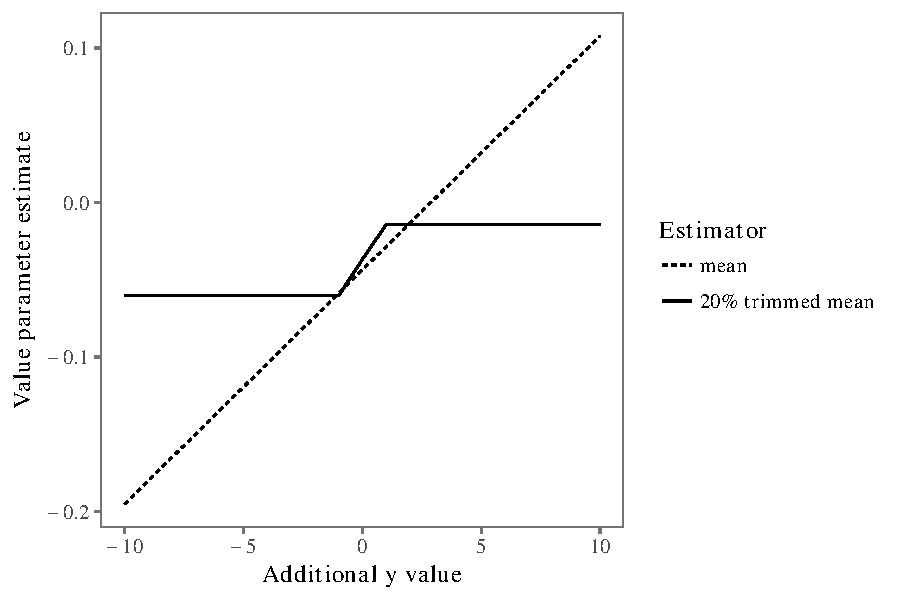
\includegraphics[scale=0.75]{IFillustration.pdf}
	\caption{The empirical influence functions of the mean and the 20\% trimmed 		mean for a random sample ($n=65$) drawn from the standard normal distribution. 
	Illustrated is the effect adding an outlier varying between $ -10 < y < 10 $ 
	on the value of the parameter estimate.}
	\label{fig:IFillustration}
	\end{minipage}

\end{center}
\end{figure}

A second measure of the robustness of an estimator is it's breakdown point (BP). 
A BP can be seen as a measure of global reliability: it measures the maximum proportion of outliers for which an estimator still returns reliable estimates \citep{Ruckstuhl2014}. 
The BP of $\mu_t$ is 0.2, that is, if less than 20\% of the values of a data set are outliers, $\mu_t$ will still return a relatively reliable estimate of the central tendency of the data \citep[p.39]{Wilcox2017}. 
By way of contrast: the BP of the mean is 0.0, i.e. one outlier can cause it's value to go to plus or minus infinity. 

The highest possible BP is 0.5, which is for example achieved by the median, however not by $\mu_t$. 
Nonetheless, in this research $\mu_t$ is preferred over robust estimators that achieve a higher BP on account of some of it's other qualities. 
Specifically, for $\mu_t$, small-sample efficiency and accurate coverage probability have been shown \citep[pp.~90-93]{Wilcox2017}.
Hence, based on the described performance of $\mu_t$, this paper proposes to use $\mu_t$ as input for \texttt{Bain} for the calculation of Bayes factors evaluating informative hypotheses, resulting in $\mathrm{AAFBF_{ROB}}$.  

Finally, as \citet[p.~5]{Wilcox2017} explains, when estimating a parameter's standard error, the method for reducing the effect of outliers should be taken into account in order to get an accurate estimate. 
For the calculation of the standard error of $\mu_t$ this paper follows the procedure described in \citet[pp.~60-64]{Wilcox2017}.

% -------------------------- Methods -------------------------- %
\section{Methods}
\label{section: Methods}
% Data description : general
Data is simulated in R \citep{R2016} from the ANOVA model:
\begin{equation}
y_{i} = \sum_{j=1}^{3}\mu_jD_{ij} + \epsilon_i,
\end{equation}
where $y_i$ is the observation on the dependent variable for person $i \ (i = 1, ..., N$), where $N$ denotes the sample size, $\mu_j$ denotes the mean of Group $j \ (j = 1, 2, 3)$, $D_{ij} = 1$ if person $i$ is in Group $j$ and $0$ otherwise and $\epsilon_{i}$ denotes the residual for person $i$, with $\epsilon_{i} \sim \mathcal{N}(0, \sigma^2)$ where $\sigma^2$ denotes the residual variance. 
From the ANOVA model, $r = 1, ..., 1,000$ data sets are sampled from two populations. In one population, 
\begin{equation}
H_1: \mu_1 = \mu_2 = \mu_3
\label{H1}
\end{equation}
is true. In this population, the groups means are chosen to be $\mu_1 = \mu_2 = \mu_3 = 0.0$ with residual variance $\sigma^2 = 1.0$.
In the other population, 
\begin{equation}
H_2: \mu_1 < \mu_2 < \mu_3
\label{H2}
\end{equation}
is true. In this population, the group means are chosen to be $\mu_1 = 0.0, \, \mu_2 = 0.5$ and $\mu_3 = 1.0$ with residual variance $\sigma^2 = 1.0$, corresponding to a medium effect size between two groups \citep{Cohen1988}. 
Data sets are sampled with sample size per group $n_j = 65$, chosen to have 80\% power to detect a difference of medium effect size between two groups with a regular ANOVA.

% Data description: outliers
With respect to the generation of outlying values, this paper focusses on one specific situation where outliers occur solely on the left side of the sample distribution, i.e. smaller values, of Group 3. 
Since the breakdown point of $\mu_t$ is known to be $0.2$, up to 20\% outliers are considered. The size of the outliers is based on the robust MAD-Median rule for detecting outliers \citep[p.101]{Wilcox2017}. 
To be more precisely, data values are replaced by values that are
\begin{equation}
\tilde{x}_3 - r \times \mathrm{MADN}_3,
\end{equation}
where $\tilde{x}_3$ is the median of Group 3 (without outliers), $r$ is a random number between 2.5 and 5 and $\mathrm{MADN}_3$ is the median absolute deviation (MAD) for Group 3 (without outliers) corrected by a normalizing constant \citep[p.~50]{Wilcox2017}.

For each data set, the OLS estimates of the population means and their covariance matrix are calculated by means of the R base function for fitting a linear model \texttt{lm()}. Additionally, for each data set, the 20 \% trimmed mean estimate is calculated by means of the R base function \texttt{mean()} for which the trimming argument is set equal to $0.2$. The standard error of the 20\% trimmed mean estimate is calculated by means of the function \texttt{trimse} from the \textsc{WRS2} package \citep*{WRS2}. 
Since in this simple ANOVA model a parameter's covariance matrix only contains it's variance, the covariance matrix of the 20\% trimmed mean estimate can be calculated by taking the standard error to the power $2$ \citep[p.60-64]{Wilcox2017}.

From the resulting distribution of OLS estimates and 20\% trimmed mean estimates, absolute bias, $\delta$, is calculated following
\begin{equation}
\delta = |(R^{-1}\sum\limits_{r=1}^{R} \hat{\mu}_r) -\mu|
\end{equation}
in which $r = 1, ..., R$ is the number of simulated data sets, where $R = 1,000$, $\hat{\mu}$ is either the OLS or 20\% trimmed mean estimate and $\mu$ is the population mean. 
Additionally, the coverage probability of the 95\% confidence interval (CI) of each estimate is calculated by counting how often the population mean is in the interval, whereby the limits of the 95\% CI are calculated following
\begin{equation}
\hat{\mu} \ \pm \ t_{0.975} \ \mathrm{SE}
\end{equation}
in which $t_{0.975}$ is the .975 quantile from a Student's t distribution with $n_j-1$ degrees of freedom for the OLS estimate and $n_j-2 \gamma n_j-1$ degrees of freedom for the 20\% trimmed mean estimate \citep[pp.~115-119]{Wilcox2017} and $\mathrm{SE}$ is the standard error of the estimate.

Subsequently, resulting estimates and their covariance matrix are fed into the \texttt{Bain} function from the \textsc{Bain} package for the calculation of the Bayes factors evaluating the informative hypotheses stated in Equations \ref{H1} and \ref{H2}, and 
\begin{equation}
H_u: \mu_1, \mu_2, \mu_3.
\label{Hu}
\end{equation}
For both estimators for each dataset, this will result in the following three types of Bayes factors
$\mathrm{BF}_{1u}$, $\mathrm{BF}_{2u}$ and $\mathrm{BF}_{12}$ evaluate the relative support in the data for $H_1$ compared to $H_u$, $H_2$ compared to $H_u$ and $H_1$ compared to $H_2$ respectively. 
Finally, from the resulting distribution of $\mathrm{BF}$, the mean $\mathrm{BF}$ will be calculated. 

% -------------------------- Results -------------------------- %

\section{Results}
\label{section: Results}
Figure \ref{Fig: biasplot} shows the relationship between the number of outliers and size of $\delta$ for both the OLS and 20\% trimmed mean estimate of the mean for Group 3 in the population where $H_1$ is true ($\mu_3 = 0.0$).  
As \ref{Fig: biasplot} shows, an increase in the number of outliers coincides with an increase in $\delta$ for both estimators. 
However, the increase in bias is considerably smaller for the 20\% trimmed mean estimator. 

\begin{figure}[t]
\begin{center}

	\begin{minipage}{.5\textheight}
	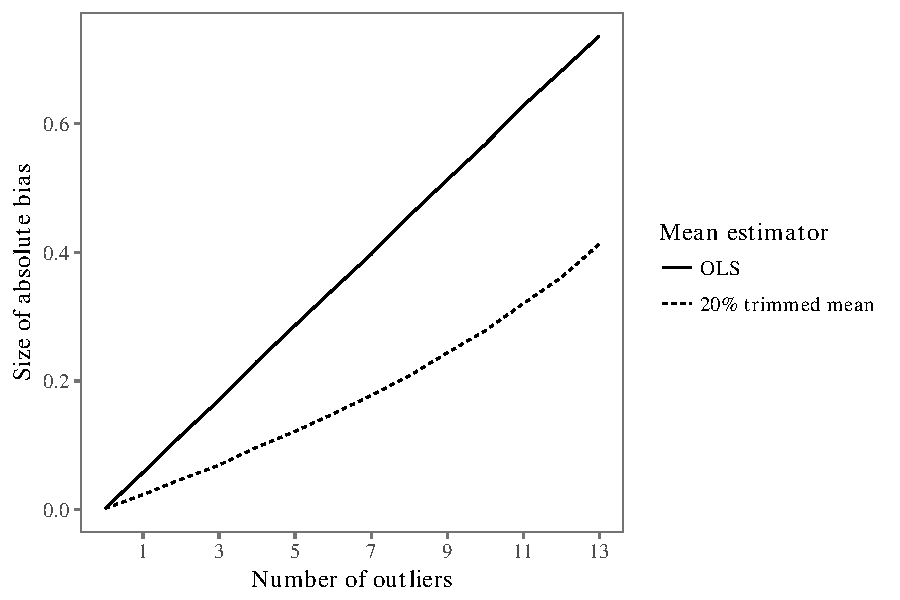
\includegraphics[scale=0.75]{partI_biasplot_pop1.pdf}
	\caption{The relationship between the number of data values replaced by
	outliers and absolute bias of the OLS and 20\% trimmed mean estimate of the
	population mean for Group 3 in the population where $H_1$ is true ($\mu_3 = 
	0.0$).}
	\label{Fig: biasplot}
	\end{minipage}
	
\end{center}
\end{figure}

Subsequently, Figure \ref{Fig: covplot} shows the relationship between the number of outliers and the coverage probability of the 95\% CI's for both the OLS and 20\% trimmed mean estimates in the population where $H_1$ is true. 
As Figure \ref{Fig: covplot} shows, an increase in the number of outliers coincides with a decrease in the coverage probability for Group 3.
For the OLS estimate, this decrease is large and already occurs with a few outliers, while for the 20\% trimmed mean estimate the decrease is considerably smaller. 
Additionally, Figure \ref{Fig: covplot} shows an increased coverage probability as a function of number of outliers for Group 1 and 2 for the OLS estimator. This is the result of an increased error variance as a consequence of outliers in combination with the equal variances assumption from the regular ANOVA, resulting in a 95\% CI that is too wide. 

\begin{figure}[t]
\begin{center}

	\begin{minipage}{.5\textheight}
	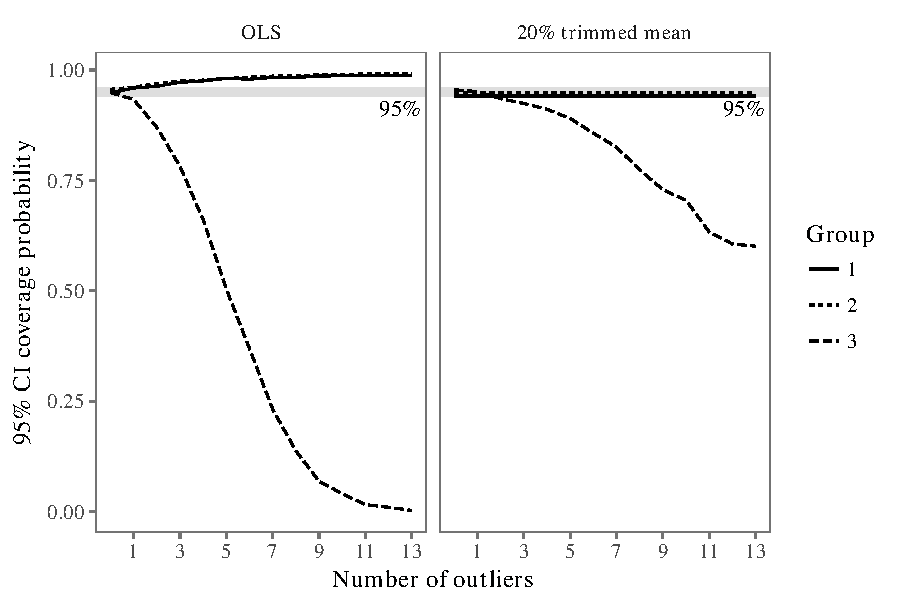
\includegraphics[scale=0.75]{partI_covplot_pop1.pdf}
	\caption{The relationship between the number of data values in Group 3
	replaced by outliers and coverage probability of the 95\% CI around the OLS
	and 20\% trimmed mean estimate of the population mean for Group 1, 2 and 3
	($n_j = 65$). Note that outliers only occur in Group 3.}
	\label{Fig: covplot}
	\end{minipage}
	
\end{center}
\end{figure}

Figure \ref{Fig: BFpop1} shows the relationship between the number of outliers and the mean size of the Bayes factors for the population where $H_1$ is true.
As Figure \ref{Fig: BFpop1} shows, the support in the data for the true hypothesis, $H_1$, compared to $H_u$, as quantified by $\mathrm{BF}_{1u}$, decreases as a function of the number of outliers for both estimators. 
This decrease is stronger for the $\mathrm{AAFBF_{OLS}}$ than for the $\mathrm{AAFBF_{ROB}}$. 
Nonetheless, also the $\mathrm{AAFBF_{OLS}}$ still indicates quite some support for the true hypothesis up to approximately 9 (14\%) outliers.
Additionally, Figure \ref{Fig: BFpop1} shows that $\mathrm{BF}_{2u}$ steadily indicates no support for $H_2$ for both estimators. 
Subsequently, Figure \ref{Fig: BFpop1} also shows a steep increase in the support in the data for $H_1$ compared to $H_2$, as quantified by $\mathrm{BF}_{12}$ for both estimators. 
This may seem somewhat contradicting with the decline in $\mathrm{BF}_{1u}$, but merely shows that with an increase in outliers the support in the data for $H_2$ decreases faster than the support in the data for $H_1$ does. 

\begin{figure}[p]
\begin{center}

	\begin{minipage}{.5\textheight}
	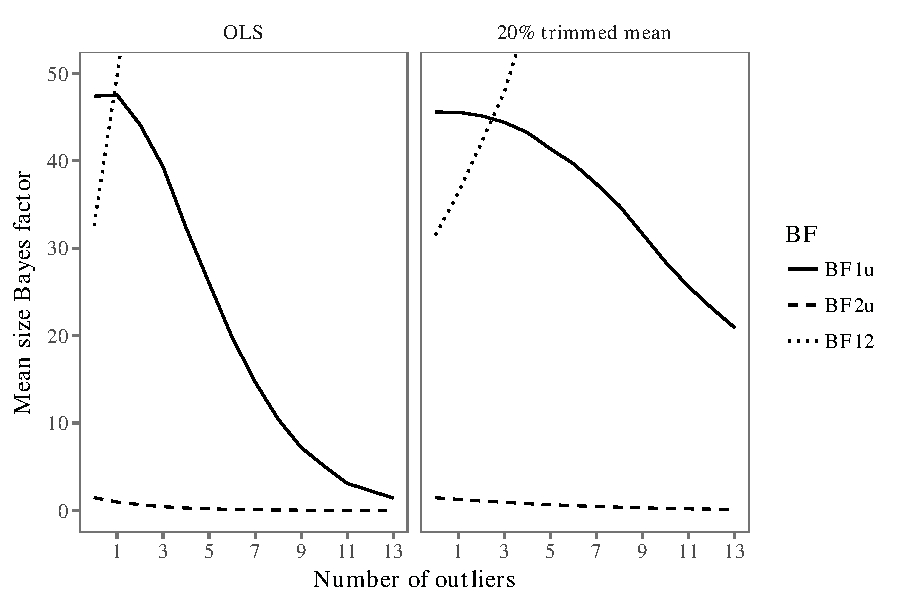
\includegraphics[scale=0.75]{partII_BF_pop1.pdf}
	\caption{The relationship between the number of data values in Group 3
	replaced by outliers and the mean size of the Bayes factors evaluating the 
	relative support in the data for the informative hypotheses stated in 
	Equations \ref{H1}, \ref{H2} and \ref{Hu}, with the OLS or 20\% trimmed mean 
	estimates as input. The underlying truth is captured in $H_1$, stated in 
	Equation \ref{H1}. Outliers in group 3 are on the left tail of the 
	distribution. Note that for the sake of visibility, the y-axis has been cut at 
	BF = 50.}
	\label{Fig: BFpop1}
	\end{minipage}
	
\end{center}
\end{figure}

\begin{figure}[p]
\begin{center}
	
	\begin{minipage}{.5\textheight}
	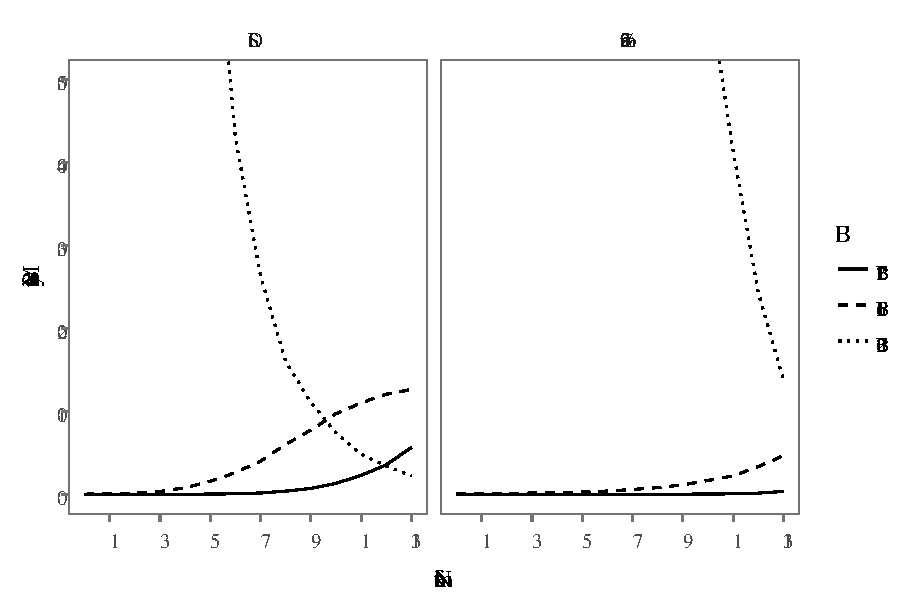
\includegraphics[scale=0.75]{partII_BF_pop2.pdf}
	\caption{The relationship between the number of data values in Group 3
	replaced by outliers and the mean size of the Bayes factors evaluating the 
	relative support in the data for the informative hypotheses stated in 
	Equations \ref{H1}, \ref{H2} and \ref{Hu}, with the OLS or 20\% trimmed mean 
	estimates as input. The underlying truth is captured in $H_2$, stated in 
	Equation \ref{H2}. Outliers in group 3 are on the left tail of the 
	distribution. Note that for the sake of visibility, the y-axis has been cut at 
	BF = 50.}
	\label{Fig: BFpop2}
	\end{minipage}
	
\end{center}
\end{figure}


Finally, Figure \ref{Fig: BFpop2} shows the relationship between the number of outliers and the mean size of the Bayes factors for the population where $H_2$ is true.
As Figure \ref{Fig: BFpop2} shows, the support in the data for the true hypothesis, $H_2$, compared to $H_u$, as quantified by $\mathrm{BF}_{2u}$, decreases as a function of the number of outliers for both estimators. 
This decreases is faster for the $\mathrm{AAFBF_{OLS}}$ than for the $\mathrm{AAFBF_{ROB}}$. 
However, again, the $\mathrm{AAFBF_{OLS}}$ still indicates quite some support for the true hypothesis up to approximately 9 (14\%) outliers.
Figure \ref{Fig: BFpop2} also shows a slow increase in the support in the data for $H_1$, a false hypothesis, compared to $H_u$, as quantified by $\mathrm{BF}_{2u}$ for both estimators. 
This increase is logically accompanied with an increase in the support in the data for $H_1$ compared to $H_2$, as quantified by $\mathrm{BF}_{12}$. 
However, for the 20\% trimmed mean estimator this increase is only small. 
In fact, both $\mathrm{BF}_{2u}$ and $\mathrm{BF}_{12}$ increase stronger for the $\mathrm{AAFBF_{OLS}}$ than for the $\mathrm{AAFBF_{ROB}}$.

% -------------------------- Discussion -------------------------- %
\section{Discussion}
\label{section: Discussion}
The results showed that the OLS estimate is less robust to outliers than the 20\% trimmed mean in terms of bias and coverage probability. 
Nonetheless, the $\mathrm{AAFBF_{ROB}}$ barely outperformed the $\mathrm{AAFBF_{OLS}}$ in terms of signalling the true hypothesis. 
An explanation for this might partly be found in Figure \ref{Fig: biasplot}. 
Figure \ref{Fig: biasplot} shows that an absolute bias of 0.5, which in this situation would be necessary to cause a different ordering of sample means, only occurs with as many as 9 outliers for the OLS estimate. 
Not coincidentally, the $\mathrm{AAFBF_{OLS}}$ breaks down with as many as 9 outliers.  
This would suggest that for the population where $H_2$ was true, the robustness of  $\mathrm{AAFBF_{OLS}}$ might partly be the result of the chosen effect sizes. 
However, for the population where $H_1$ is true, the chosen effect sizes should not be of influence. 
Hence, the exact influence of effect sizes on the size of the $\mathrm{AAFBF}$ needs to be further investigated. 

In conclusion, the $\mathrm{AAFBF_{OLS}}$ estimates seems quite robust in the situations simulated in this research. 
However, the $\mathrm{AAFBF_{ROB}}$ estimates performs even better. In addition, some sample and population characteristics, like effect size or direction of outliers, might reinforce the adverse effect of outliers on the behaviour of the $\mathrm{AAFBF_{OLS}}$. 
Therefore, we would advise researchers that worry about the potential impact of outliers in their dataset to use a robust estimator, like the 20\% trimmed mean, for the calculation of the $\mathrm{AAFBF}$. 
Future research should provide us with more clarity with regard the effect of the interaction between sample and population characteristics and outliers on the behaviour of Bayes factors. 

% -------------------------- References -------------------------- %
\bibliographystyle{apacite}
\bibliography{research_paper}

\end{document}